\begin{figure}[ht]

\centering

\begin{subfigure}{0.33\textwidth}
\centering
\begin{minipage}{\textwidth}
\tikzsetnextfilename{ASSTheta1}

\centering
\resizebox{1\textwidth}{!}{
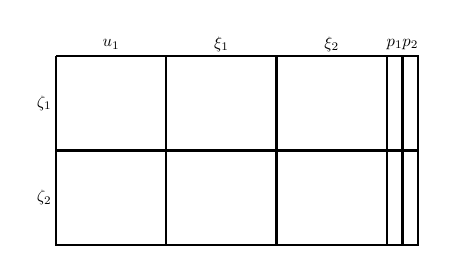
\begin{tikzpicture}[yscale=-1] 

\pgfmathsetmacro{\nt}{7};% time points
\pgfmathsetmacro{\ntm}{\nt-1};
\pgfmathsetmacro{\nu}{1}; % controls
\pgfmathsetmacro{\nx}{2}; % states
\pgfmathsetmacro{\np}{2}; % parameters
\pgfmathsetmacro{\nc}{\nu + \nx}; % total continuous

%% control labels
\foreach \k in {1,...,\nu}{
	\pgfmathsetmacro{\x}{0.2*\nt*\k - 0.2/2*(\nt-1)};
	\node () at (\x,-0.05) {\scalebox{0.6}{$u_{\k}$}};
}

%% state labels
\foreach \k in {1,...,\nx}{
	\pgfmathsetmacro{\x}{0.2*\nt*\k + 0.2*\nu*\nt - 0.2/2*(\nt-1)};
	\node () at (\x,-0.05) {\scalebox{0.6}{$\xi_{\k}$}};
}

%% parameter labels
\foreach \k in {1,...,\np}{
	\pgfmathsetmacro{\x}{0.2*\k + 0.2*\nu*\nt + 0.2*\nx*\nt};
	\node () at (\x,-0.05) {\scalebox{0.6}{$p_{\k}$}};
}

%% defects
\foreach \k in {1,...,\nx}{
	\pgfmathsetmacro{\x}{0.2*\ntm*\k - 0.2/2*(\ntm-1)};
	\node () at (-0.05,\x) {\scalebox{0.6}{$\zeta_{\k}$}};
}


%% controls
\foreach \k in {1,...,\nu}{
	\foreach \j in {1,...,\nx}{
		\foreach \i in {1,...,\ntm}{ 
        	\pgfmathsetmacro{\kk}{\k-1};
            \pgfmathsetmacro{\jj}{\j-1};
        	\pgfmathsetmacro{\x}{0.2*\i + 0.2*\kk*\nt};
            \pgfmathsetmacro{\y}{0.2*\i + 0.2*\jj*\ntm};
        	\node () at (\x,\y) {\mysparsesymbol};
            \node () at (\x+0.2,\y) {\mysparsesymbol};
} 
    \pgfmathsetmacro{\kk}{\k-1};
    \pgfmathsetmacro{\jj}{\j-1};
    \pgfmathsetmacro{\x}{0.2*\kk*\nt + 0.1};
    \pgfmathsetmacro{\y}{0.2*\jj*\ntm + 0.1};
	\draw[\mysparseboxcolor,thick](\x,\y) -- (\x+0.2*\nt,\y) -- (\x+0.2*\nt,\y+0.2*\ntm) -- (\x,\y+0.2*\ntm) -- (\x,\y);
} }

%% states
\foreach \k in {1,...,\nx}{
	\foreach \j in {1,...,\nx}{
		\foreach \i in {1,...,\ntm}{ 
        	\pgfmathsetmacro{\kk}{\k-1};
            \pgfmathsetmacro{\jj}{\j-1};
        	\pgfmathsetmacro{\x}{0.2*\i + 0.2*\nu*\nt + 0.2*\kk*\nt};
            \pgfmathsetmacro{\y}{0.2*\i + 0.2*\jj*\ntm};
        	\node () at (\x,\y) {\mysparsesymbol};
            \node () at (\x+0.2,\y) {\mysparsesymbol};
} 
    \pgfmathsetmacro{\kk}{\k-1};
    \pgfmathsetmacro{\jj}{\j-1};
    \pgfmathsetmacro{\x}{0.2*\kk*\nt + 0.2*\nu*\nt + 0.1};
    \pgfmathsetmacro{\y}{0.2*\jj*\ntm + 0.1};
	\draw[\mysparseboxcolor,thick](\x,\y) -- (\x+0.2*\nt,\y) -- (\x+0.2*\nt,\y+0.2*\ntm) -- (\x,\y+0.2*\ntm) -- (\x,\y);
} }

%% states and parameters
\foreach \k in {1,...,\np}{
	\foreach \j in {1,...,\nx}{
		\foreach \i in {1,...,\ntm}{ 
        	\pgfmathsetmacro{\kk}{\k-1};
            \pgfmathsetmacro{\jj}{\j-1};
        	\node () at ( 0.2*\k + 0.2*\nx*\nt + 0.2*\nu*\nt, 0.2*\i + 0.2*\jj*\ntm ) {\mysparsesymbol};
} 
    \pgfmathsetmacro{\kk}{\k-1};
    \pgfmathsetmacro{\jj}{\j-1};
    \pgfmathsetmacro{\x}{0.2*\kk + 0.2*\nx*\nt + 0.2*\nu*\nt + 0.1};
    \pgfmathsetmacro{\y}{0.2*\jj*\ntm+ 0.1};
	\draw[\mysparseboxcolor,thick](\x,\y) -- (\x+0.2,\y) -- (\x+0.2,\y+0.2*\ntm) -- (\x,\y+0.2*\ntm) -- (\x,\y);
} }

%% states
\foreach \k in {1,...,\nx}{
	\foreach \j in {1,...,\nx}{
		\foreach \i in {1,...,\ntm}{ 
        	\pgfmathsetmacro{\kk}{\k-1};
            \pgfmathsetmacro{\jj}{\j-1};
        	\pgfmathsetmacro{\x}{0.2*\i + 0.2*\nu*\nt + 0.2*\kk*\nt};
            \pgfmathsetmacro{\y}{0.2*\i + 0.2*\jj*\ntm};
        	\node () at (\x,\y) {\mytemp};
} } }

\end{tikzpicture}
}
\end{minipage}
\caption{$\bm{\theta}_1$ terms.}
% \label{fig:}
\end{subfigure}%
\begin{subfigure}{0.33\textwidth}
\centering
\begin{minipage}{\textwidth}
\tikzsetnextfilename{ASSTheta2}

\centering
\resizebox{1\textwidth}{!}{
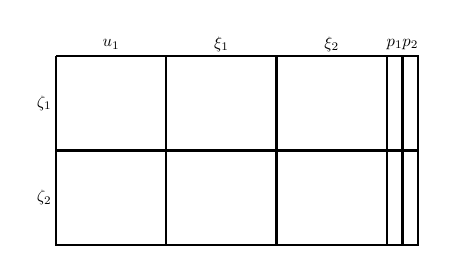
\begin{tikzpicture}[yscale=-1] 

\pgfmathsetmacro{\nt}{7};% time points
\pgfmathsetmacro{\ntm}{\nt-1};
\pgfmathsetmacro{\nu}{1}; % controls
\pgfmathsetmacro{\nx}{2}; % states
\pgfmathsetmacro{\np}{2}; % parameters
\pgfmathsetmacro{\nc}{\nu + \nx}; % total continuous

%% control labels
\foreach \k in {1,...,\nu}{
	\pgfmathsetmacro{\x}{0.2*\nt*\k - 0.2/2*(\nt-1)};
	\node () at (\x,-0.05) {\scalebox{0.6}{$u_{\k}$}};
}

%% state labels
\foreach \k in {1,...,\nx}{
	\pgfmathsetmacro{\x}{0.2*\nt*\k + 0.2*\nu*\nt - 0.2/2*(\nt-1)};
	\node () at (\x,-0.05) {\scalebox{0.6}{$\xi_{\k}$}};
}

%% parameter labels
\foreach \k in {1,...,\np}{
	\pgfmathsetmacro{\x}{0.2*\k + 0.2*\nu*\nt + 0.2*\nx*\nt};
	\node () at (\x,-0.05) {\scalebox{0.6}{$p_{\k}$}};
}

%% defects
\foreach \k in {1,...,\nx}{
	\pgfmathsetmacro{\x}{0.2*\ntm*\k - 0.2/2*(\ntm-1)};
	\node () at (-0.05,\x) {\scalebox{0.6}{$\zeta_{\k}$}};
}


%% controls
\foreach \k in {1,...,\nu}{
	\foreach \j in {1,...,\nx}{
		\foreach \i in {1,...,\ntm}{ 
        	\pgfmathsetmacro{\kk}{\k-1};
            \pgfmathsetmacro{\jj}{\j-1};
        	\pgfmathsetmacro{\x}{0.2*\i + 0.2*\kk*\nt};
            \pgfmathsetmacro{\y}{0.2*\i + 0.2*\jj*\ntm};
        	\node () at (\x,\y) {\mysparsesymbol};
            \node () at (\x+0.2,\y) {\mysparsesymbol};
} 
    \pgfmathsetmacro{\kk}{\k-1};
    \pgfmathsetmacro{\jj}{\j-1};
    \pgfmathsetmacro{\x}{0.2*\kk*\nt + 0.1};
    \pgfmathsetmacro{\y}{0.2*\jj*\ntm + 0.1};
	\draw[\mysparseboxcolor,thick](\x,\y) -- (\x+0.2*\nt,\y) -- (\x+0.2*\nt,\y+0.2*\ntm) -- (\x,\y+0.2*\ntm) -- (\x,\y);
} }

%% states
\foreach \k in {1,...,\nx}{
	\foreach \j in {1,...,\nx}{
		\foreach \i in {1,...,\ntm}{ 
        	\pgfmathsetmacro{\kk}{\k-1};
            \pgfmathsetmacro{\jj}{\j-1};
        	\pgfmathsetmacro{\x}{0.2*\i + 0.2*\nu*\nt + 0.2*\kk*\nt};
            \pgfmathsetmacro{\y}{0.2*\i + 0.2*\jj*\ntm};
        	\node () at (\x,\y) {\mysparsesymbol};
            \node () at (\x+0.2,\y) {\mysparsesymbol};
} 
    \pgfmathsetmacro{\kk}{\k-1};
    \pgfmathsetmacro{\jj}{\j-1};
    \pgfmathsetmacro{\x}{0.2*\kk*\nt + 0.2*\nu*\nt + 0.1};
    \pgfmathsetmacro{\y}{0.2*\jj*\ntm + 0.1};
	\draw[\mysparseboxcolor,thick](\x,\y) -- (\x+0.2*\nt,\y) -- (\x+0.2*\nt,\y+0.2*\ntm) -- (\x,\y+0.2*\ntm) -- (\x,\y);
} }

%% states and parameters
\foreach \k in {1,...,\np}{
	\foreach \j in {1,...,\nx}{
		\foreach \i in {1,...,\ntm}{ 
        	\pgfmathsetmacro{\kk}{\k-1};
            \pgfmathsetmacro{\jj}{\j-1};
        	\node () at ( 0.2*\k + 0.2*\nx*\nt + 0.2*\nu*\nt, 0.2*\i + 0.2*\jj*\ntm ) {\mysparsesymbol};
} 
    \pgfmathsetmacro{\kk}{\k-1};
    \pgfmathsetmacro{\jj}{\j-1};
    \pgfmathsetmacro{\x}{0.2*\kk + 0.2*\nx*\nt + 0.2*\nu*\nt + 0.1};
    \pgfmathsetmacro{\y}{0.2*\jj*\ntm+ 0.1};
	\draw[\mysparseboxcolor,thick](\x,\y) -- (\x+0.2,\y) -- (\x+0.2,\y+0.2*\ntm) -- (\x,\y+0.2*\ntm) -- (\x,\y);
} }

%% states
\foreach \k in {1,...,\nx}{
	\foreach \j in {1,...,\nx}{
		\foreach \i in {1,...,\ntm}{ 
        	\pgfmathsetmacro{\kk}{\k-1};
            \pgfmathsetmacro{\jj}{\j-1};
        	\pgfmathsetmacro{\x}{0.2*\i + 0.2*\nu*\nt + 0.2*\kk*\nt};
            \pgfmathsetmacro{\y}{0.2*\i + 0.2*\jj*\ntm};
            \node () at (\x+0.2,\y) {\mytemp};
} } }

\end{tikzpicture}
}
\end{minipage}
\caption{$\bm{\theta}_2$ terms.}
% \label{fig:}
\end{subfigure}%
\begin{subfigure}{0.33\textwidth}
\centering
\begin{minipage}{\textwidth}
\tikzsetnextfilename{ASSTheta3}

\centering
\resizebox{1\textwidth}{!}{
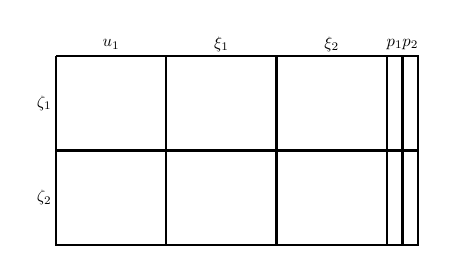
\begin{tikzpicture}[yscale=-1] 

\pgfmathsetmacro{\nt}{7};% time points
\pgfmathsetmacro{\ntm}{\nt-1};
\pgfmathsetmacro{\nu}{1}; % controls
\pgfmathsetmacro{\nx}{2}; % states
\pgfmathsetmacro{\np}{2}; % parameters
\pgfmathsetmacro{\nc}{\nu + \nx}; % total continuous

%% control labels
\foreach \k in {1,...,\nu}{
	\pgfmathsetmacro{\x}{0.2*\nt*\k - 0.2/2*(\nt-1)};
	\node () at (\x,-0.05) {\scalebox{0.6}{$u_{\k}$}};
}

%% state labels
\foreach \k in {1,...,\nx}{
	\pgfmathsetmacro{\x}{0.2*\nt*\k + 0.2*\nu*\nt - 0.2/2*(\nt-1)};
	\node () at (\x,-0.05) {\scalebox{0.6}{$\xi_{\k}$}};
}

%% parameter labels
\foreach \k in {1,...,\np}{
	\pgfmathsetmacro{\x}{0.2*\k + 0.2*\nu*\nt + 0.2*\nx*\nt};
	\node () at (\x,-0.05) {\scalebox{0.6}{$p_{\k}$}};
}

%% defects
\foreach \k in {1,...,\nx}{
	\pgfmathsetmacro{\x}{0.2*\ntm*\k - 0.2/2*(\ntm-1)};
	\node () at (-0.05,\x) {\scalebox{0.6}{$\zeta_{\k}$}};
}


%% controls
\foreach \k in {1,...,\nu}{
	\foreach \j in {1,...,\nx}{
		\foreach \i in {1,...,\ntm}{ 
        	\pgfmathsetmacro{\kk}{\k-1};
            \pgfmathsetmacro{\jj}{\j-1};
        	\pgfmathsetmacro{\x}{0.2*\i + 0.2*\kk*\nt};
            \pgfmathsetmacro{\y}{0.2*\i + 0.2*\jj*\ntm};
        	\node () at (\x,\y) {\mysparsesymbol};
            \node () at (\x+0.2,\y) {\mysparsesymbol};
} 
    \pgfmathsetmacro{\kk}{\k-1};
    \pgfmathsetmacro{\jj}{\j-1};
    \pgfmathsetmacro{\x}{0.2*\kk*\nt + 0.1};
    \pgfmathsetmacro{\y}{0.2*\jj*\ntm + 0.1};
	\draw[\mysparseboxcolor,thick](\x,\y) -- (\x+0.2*\nt,\y) -- (\x+0.2*\nt,\y+0.2*\ntm) -- (\x,\y+0.2*\ntm) -- (\x,\y);
} }

%% states
\foreach \k in {1,...,\nx}{
	\foreach \j in {1,...,\nx}{
		\foreach \i in {1,...,\ntm}{ 
        	\pgfmathsetmacro{\kk}{\k-1};
            \pgfmathsetmacro{\jj}{\j-1};
        	\pgfmathsetmacro{\x}{0.2*\i + 0.2*\nu*\nt + 0.2*\kk*\nt};
            \pgfmathsetmacro{\y}{0.2*\i + 0.2*\jj*\ntm};
        	\node () at (\x,\y) {\mysparsesymbol};
            \node () at (\x+0.2,\y) {\mysparsesymbol};
} 
    \pgfmathsetmacro{\kk}{\k-1};
    \pgfmathsetmacro{\jj}{\j-1};
    \pgfmathsetmacro{\x}{0.2*\kk*\nt + 0.2*\nu*\nt + 0.1};
    \pgfmathsetmacro{\y}{0.2*\jj*\ntm + 0.1};
	\draw[\mysparseboxcolor,thick](\x,\y) -- (\x+0.2*\nt,\y) -- (\x+0.2*\nt,\y+0.2*\ntm) -- (\x,\y+0.2*\ntm) -- (\x,\y);
} }

%% states and parameters
\foreach \k in {1,...,\np}{
	\foreach \j in {1,...,\nx}{
		\foreach \i in {1,...,\ntm}{ 
        	\pgfmathsetmacro{\kk}{\k-1};
            \pgfmathsetmacro{\jj}{\j-1};
        	\node () at ( 0.2*\k + 0.2*\nx*\nt + 0.2*\nu*\nt, 0.2*\i + 0.2*\jj*\ntm ) {\mysparsesymbol};
} 
    \pgfmathsetmacro{\kk}{\k-1};
    \pgfmathsetmacro{\jj}{\j-1};
    \pgfmathsetmacro{\x}{0.2*\kk + 0.2*\nx*\nt + 0.2*\nu*\nt + 0.1};
    \pgfmathsetmacro{\y}{0.2*\jj*\ntm+ 0.1};
	\draw[\mysparseboxcolor,thick](\x,\y) -- (\x+0.2,\y) -- (\x+0.2,\y+0.2*\ntm) -- (\x,\y+0.2*\ntm) -- (\x,\y);
} }

%% controls
\foreach \k in {1,...,\nu}{
	\foreach \j in {1,...,\nx}{
		\foreach \i in {1,...,\ntm}{ 
        	\pgfmathsetmacro{\kk}{\k-1};
            \pgfmathsetmacro{\jj}{\j-1};
        	\pgfmathsetmacro{\x}{0.2*\i + 0.2*\kk*\nt};
            \pgfmathsetmacro{\y}{0.2*\i + 0.2*\jj*\ntm};
        	\node () at (\x,\y) {\mytemp};
} } }

\end{tikzpicture}
}
\end{minipage}
\caption{$\bm{\theta}_3$ terms.}
% \label{fig:}
\end{subfigure}%

\begin{subfigure}{0.33\textwidth}
\centering
\begin{minipage}{\textwidth}
\tikzsetnextfilename{ASSTheta4}

\centering
\resizebox{1\textwidth}{!}{
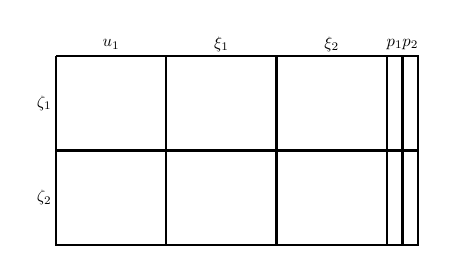
\begin{tikzpicture}[yscale=-1] 

\pgfmathsetmacro{\nt}{7};% time points
\pgfmathsetmacro{\ntm}{\nt-1};
\pgfmathsetmacro{\nu}{1}; % controls
\pgfmathsetmacro{\nx}{2}; % states
\pgfmathsetmacro{\np}{2}; % parameters
\pgfmathsetmacro{\nc}{\nu + \nx}; % total continuous

%% control labels
\foreach \k in {1,...,\nu}{
	\pgfmathsetmacro{\x}{0.2*\nt*\k - 0.2/2*(\nt-1)};
	\node () at (\x,-0.05) {\scalebox{0.6}{$u_{\k}$}};
}

%% state labels
\foreach \k in {1,...,\nx}{
	\pgfmathsetmacro{\x}{0.2*\nt*\k + 0.2*\nu*\nt - 0.2/2*(\nt-1)};
	\node () at (\x,-0.05) {\scalebox{0.6}{$\xi_{\k}$}};
}

%% parameter labels
\foreach \k in {1,...,\np}{
	\pgfmathsetmacro{\x}{0.2*\k + 0.2*\nu*\nt + 0.2*\nx*\nt};
	\node () at (\x,-0.05) {\scalebox{0.6}{$p_{\k}$}};
}

%% defects
\foreach \k in {1,...,\nx}{
	\pgfmathsetmacro{\x}{0.2*\ntm*\k - 0.2/2*(\ntm-1)};
	\node () at (-0.05,\x) {\scalebox{0.6}{$\zeta_{\k}$}};
}


%% controls
\foreach \k in {1,...,\nu}{
	\foreach \j in {1,...,\nx}{
		\foreach \i in {1,...,\ntm}{ 
        	\pgfmathsetmacro{\kk}{\k-1};
            \pgfmathsetmacro{\jj}{\j-1};
        	\pgfmathsetmacro{\x}{0.2*\i + 0.2*\kk*\nt};
            \pgfmathsetmacro{\y}{0.2*\i + 0.2*\jj*\ntm};
        	\node () at (\x,\y) {\mysparsesymbol};
            \node () at (\x+0.2,\y) {\mysparsesymbol};
} 
    \pgfmathsetmacro{\kk}{\k-1};
    \pgfmathsetmacro{\jj}{\j-1};
    \pgfmathsetmacro{\x}{0.2*\kk*\nt + 0.1};
    \pgfmathsetmacro{\y}{0.2*\jj*\ntm + 0.1};
	\draw[\mysparseboxcolor,thick](\x,\y) -- (\x+0.2*\nt,\y) -- (\x+0.2*\nt,\y+0.2*\ntm) -- (\x,\y+0.2*\ntm) -- (\x,\y);
} }

%% states
\foreach \k in {1,...,\nx}{
	\foreach \j in {1,...,\nx}{
		\foreach \i in {1,...,\ntm}{ 
        	\pgfmathsetmacro{\kk}{\k-1};
            \pgfmathsetmacro{\jj}{\j-1};
        	\pgfmathsetmacro{\x}{0.2*\i + 0.2*\nu*\nt + 0.2*\kk*\nt};
            \pgfmathsetmacro{\y}{0.2*\i + 0.2*\jj*\ntm};
        	\node () at (\x,\y) {\mysparsesymbol};
            \node () at (\x+0.2,\y) {\mysparsesymbol};
} 
    \pgfmathsetmacro{\kk}{\k-1};
    \pgfmathsetmacro{\jj}{\j-1};
    \pgfmathsetmacro{\x}{0.2*\kk*\nt + 0.2*\nu*\nt + 0.1};
    \pgfmathsetmacro{\y}{0.2*\jj*\ntm + 0.1};
	\draw[\mysparseboxcolor,thick](\x,\y) -- (\x+0.2*\nt,\y) -- (\x+0.2*\nt,\y+0.2*\ntm) -- (\x,\y+0.2*\ntm) -- (\x,\y);
} }

%% states and parameters
\foreach \k in {1,...,\np}{
	\foreach \j in {1,...,\nx}{
		\foreach \i in {1,...,\ntm}{ 
        	\pgfmathsetmacro{\kk}{\k-1};
            \pgfmathsetmacro{\jj}{\j-1};
        	\node () at ( 0.2*\k + 0.2*\nx*\nt + 0.2*\nu*\nt, 0.2*\i + 0.2*\jj*\ntm ) {\mysparsesymbol};
} 
    \pgfmathsetmacro{\kk}{\k-1};
    \pgfmathsetmacro{\jj}{\j-1};
    \pgfmathsetmacro{\x}{0.2*\kk + 0.2*\nx*\nt + 0.2*\nu*\nt + 0.1};
    \pgfmathsetmacro{\y}{0.2*\jj*\ntm+ 0.1};
	\draw[\mysparseboxcolor,thick](\x,\y) -- (\x+0.2,\y) -- (\x+0.2,\y+0.2*\ntm) -- (\x,\y+0.2*\ntm) -- (\x,\y);
} }

%% controls
\foreach \k in {1,...,\nu}{
	\foreach \j in {1,...,\nx}{
		\foreach \i in {1,...,\ntm}{ 
        	\pgfmathsetmacro{\kk}{\k-1};
            \pgfmathsetmacro{\jj}{\j-1};
        	\pgfmathsetmacro{\x}{0.2*\i + 0.2*\kk*\nt};
            \pgfmathsetmacro{\y}{0.2*\i + 0.2*\jj*\ntm};
            \node () at (\x+0.2,\y) {\mytemp};
} } }

\end{tikzpicture}
}
\end{minipage}
\caption{$\bm{\theta}_4$ terms.}
% \label{fig:}
\end{subfigure}%
\begin{subfigure}{0.33\textwidth}
\centering
\begin{minipage}{\textwidth}
\tikzsetnextfilename{ASSTheta5}

\centering
\resizebox{1\textwidth}{!}{
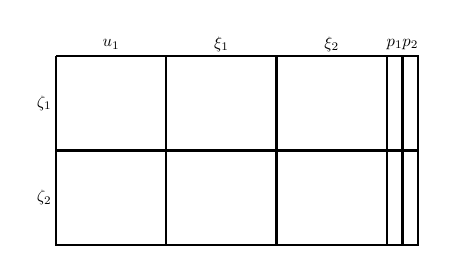
\begin{tikzpicture}[yscale=-1] 

\pgfmathsetmacro{\nt}{7};% time points
\pgfmathsetmacro{\ntm}{\nt-1};
\pgfmathsetmacro{\nu}{1}; % controls
\pgfmathsetmacro{\nx}{2}; % states
\pgfmathsetmacro{\np}{2}; % parameters
\pgfmathsetmacro{\nc}{\nu + \nx}; % total continuous

%% control labels
\foreach \k in {1,...,\nu}{
	\pgfmathsetmacro{\x}{0.2*\nt*\k - 0.2/2*(\nt-1)};
	\node () at (\x,-0.05) {\scalebox{0.6}{$u_{\k}$}};
}

%% state labels
\foreach \k in {1,...,\nx}{
	\pgfmathsetmacro{\x}{0.2*\nt*\k + 0.2*\nu*\nt - 0.2/2*(\nt-1)};
	\node () at (\x,-0.05) {\scalebox{0.6}{$\xi_{\k}$}};
}

%% parameter labels
\foreach \k in {1,...,\np}{
	\pgfmathsetmacro{\x}{0.2*\k + 0.2*\nu*\nt + 0.2*\nx*\nt};
	\node () at (\x,-0.05) {\scalebox{0.6}{$p_{\k}$}};
}

%% defects
\foreach \k in {1,...,\nx}{
	\pgfmathsetmacro{\x}{0.2*\ntm*\k - 0.2/2*(\ntm-1)};
	\node () at (-0.05,\x) {\scalebox{0.6}{$\zeta_{\k}$}};
}


%% controls
\foreach \k in {1,...,\nu}{
	\foreach \j in {1,...,\nx}{
		\foreach \i in {1,...,\ntm}{ 
        	\pgfmathsetmacro{\kk}{\k-1};
            \pgfmathsetmacro{\jj}{\j-1};
        	\pgfmathsetmacro{\x}{0.2*\i + 0.2*\kk*\nt};
            \pgfmathsetmacro{\y}{0.2*\i + 0.2*\jj*\ntm};
        	\node () at (\x,\y) {\mysparsesymbol};
            \node () at (\x+0.2,\y) {\mysparsesymbol};
} 
    \pgfmathsetmacro{\kk}{\k-1};
    \pgfmathsetmacro{\jj}{\j-1};
    \pgfmathsetmacro{\x}{0.2*\kk*\nt + 0.1};
    \pgfmathsetmacro{\y}{0.2*\jj*\ntm + 0.1};
	\draw[\mysparseboxcolor,thick](\x,\y) -- (\x+0.2*\nt,\y) -- (\x+0.2*\nt,\y+0.2*\ntm) -- (\x,\y+0.2*\ntm) -- (\x,\y);
} }

%% states
\foreach \k in {1,...,\nx}{
	\foreach \j in {1,...,\nx}{
		\foreach \i in {1,...,\ntm}{ 
        	\pgfmathsetmacro{\kk}{\k-1};
            \pgfmathsetmacro{\jj}{\j-1};
        	\pgfmathsetmacro{\x}{0.2*\i + 0.2*\nu*\nt + 0.2*\kk*\nt};
            \pgfmathsetmacro{\y}{0.2*\i + 0.2*\jj*\ntm};
        	\node () at (\x,\y) {\mysparsesymbol};
            \node () at (\x+0.2,\y) {\mysparsesymbol};
} 
    \pgfmathsetmacro{\kk}{\k-1};
    \pgfmathsetmacro{\jj}{\j-1};
    \pgfmathsetmacro{\x}{0.2*\kk*\nt + 0.2*\nu*\nt + 0.1};
    \pgfmathsetmacro{\y}{0.2*\jj*\ntm + 0.1};
	\draw[\mysparseboxcolor,thick](\x,\y) -- (\x+0.2*\nt,\y) -- (\x+0.2*\nt,\y+0.2*\ntm) -- (\x,\y+0.2*\ntm) -- (\x,\y);
} }

%% states and parameters
\foreach \k in {1,...,\np}{
	\foreach \j in {1,...,\nx}{
		\foreach \i in {1,...,\ntm}{ 
        	\pgfmathsetmacro{\kk}{\k-1};
            \pgfmathsetmacro{\jj}{\j-1};
        	\node () at ( 0.2*\k + 0.2*\nx*\nt + 0.2*\nu*\nt, 0.2*\i + 0.2*\jj*\ntm ) {\mysparsesymbol};
} 
    \pgfmathsetmacro{\kk}{\k-1};
    \pgfmathsetmacro{\jj}{\j-1};
    \pgfmathsetmacro{\x}{0.2*\kk + 0.2*\nx*\nt + 0.2*\nu*\nt + 0.1};
    \pgfmathsetmacro{\y}{0.2*\jj*\ntm+ 0.1};
	\draw[\mysparseboxcolor,thick](\x,\y) -- (\x+0.2,\y) -- (\x+0.2,\y+0.2*\ntm) -- (\x,\y+0.2*\ntm) -- (\x,\y);
} }

%% states and parameters
\foreach \k in {1,...,\np}{
	\foreach \j in {1,...,\nx}{
		\foreach \i in {1,...,\ntm}{ 
        	\pgfmathsetmacro{\kk}{\k-1};
            \pgfmathsetmacro{\jj}{\j-1};
        	\node () at ( 0.2*\k + 0.2*\nx*\nt + 0.2*\nu*\nt, 0.2*\i + 0.2*\jj*\ntm ) {\mytemp};
} } }

\end{tikzpicture}
}
\end{minipage}
\caption{$\bm{\theta}_5$ terms.}
% \label{fig:}
\end{subfigure}%

\caption{Sparsity pattern of $\mathbf{A}_{e1}$ matrix for the defect constraints using a single-step method.}\label{fig:figsparsityASS}
\end{figure}


% \begin{figure}[h]

% \centering

% \subfloat[(a) $\bm{\theta}_1$ terms.]{
% 	\begin{minipage}{0.33\textwidth}
% 	\tikzsetnextfilename{ASSTheta1}

\centering
\resizebox{1\textwidth}{!}{
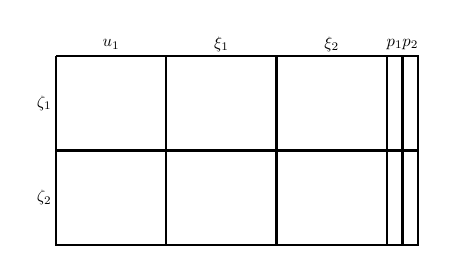
\begin{tikzpicture}[yscale=-1] 

\pgfmathsetmacro{\nt}{7};% time points
\pgfmathsetmacro{\ntm}{\nt-1};
\pgfmathsetmacro{\nu}{1}; % controls
\pgfmathsetmacro{\nx}{2}; % states
\pgfmathsetmacro{\np}{2}; % parameters
\pgfmathsetmacro{\nc}{\nu + \nx}; % total continuous

%% control labels
\foreach \k in {1,...,\nu}{
	\pgfmathsetmacro{\x}{0.2*\nt*\k - 0.2/2*(\nt-1)};
	\node () at (\x,-0.05) {\scalebox{0.6}{$u_{\k}$}};
}

%% state labels
\foreach \k in {1,...,\nx}{
	\pgfmathsetmacro{\x}{0.2*\nt*\k + 0.2*\nu*\nt - 0.2/2*(\nt-1)};
	\node () at (\x,-0.05) {\scalebox{0.6}{$\xi_{\k}$}};
}

%% parameter labels
\foreach \k in {1,...,\np}{
	\pgfmathsetmacro{\x}{0.2*\k + 0.2*\nu*\nt + 0.2*\nx*\nt};
	\node () at (\x,-0.05) {\scalebox{0.6}{$p_{\k}$}};
}

%% defects
\foreach \k in {1,...,\nx}{
	\pgfmathsetmacro{\x}{0.2*\ntm*\k - 0.2/2*(\ntm-1)};
	\node () at (-0.05,\x) {\scalebox{0.6}{$\zeta_{\k}$}};
}


%% controls
\foreach \k in {1,...,\nu}{
	\foreach \j in {1,...,\nx}{
		\foreach \i in {1,...,\ntm}{ 
        	\pgfmathsetmacro{\kk}{\k-1};
            \pgfmathsetmacro{\jj}{\j-1};
        	\pgfmathsetmacro{\x}{0.2*\i + 0.2*\kk*\nt};
            \pgfmathsetmacro{\y}{0.2*\i + 0.2*\jj*\ntm};
        	\node () at (\x,\y) {\mysparsesymbol};
            \node () at (\x+0.2,\y) {\mysparsesymbol};
} 
    \pgfmathsetmacro{\kk}{\k-1};
    \pgfmathsetmacro{\jj}{\j-1};
    \pgfmathsetmacro{\x}{0.2*\kk*\nt + 0.1};
    \pgfmathsetmacro{\y}{0.2*\jj*\ntm + 0.1};
	\draw[\mysparseboxcolor,thick](\x,\y) -- (\x+0.2*\nt,\y) -- (\x+0.2*\nt,\y+0.2*\ntm) -- (\x,\y+0.2*\ntm) -- (\x,\y);
} }

%% states
\foreach \k in {1,...,\nx}{
	\foreach \j in {1,...,\nx}{
		\foreach \i in {1,...,\ntm}{ 
        	\pgfmathsetmacro{\kk}{\k-1};
            \pgfmathsetmacro{\jj}{\j-1};
        	\pgfmathsetmacro{\x}{0.2*\i + 0.2*\nu*\nt + 0.2*\kk*\nt};
            \pgfmathsetmacro{\y}{0.2*\i + 0.2*\jj*\ntm};
        	\node () at (\x,\y) {\mysparsesymbol};
            \node () at (\x+0.2,\y) {\mysparsesymbol};
} 
    \pgfmathsetmacro{\kk}{\k-1};
    \pgfmathsetmacro{\jj}{\j-1};
    \pgfmathsetmacro{\x}{0.2*\kk*\nt + 0.2*\nu*\nt + 0.1};
    \pgfmathsetmacro{\y}{0.2*\jj*\ntm + 0.1};
	\draw[\mysparseboxcolor,thick](\x,\y) -- (\x+0.2*\nt,\y) -- (\x+0.2*\nt,\y+0.2*\ntm) -- (\x,\y+0.2*\ntm) -- (\x,\y);
} }

%% states and parameters
\foreach \k in {1,...,\np}{
	\foreach \j in {1,...,\nx}{
		\foreach \i in {1,...,\ntm}{ 
        	\pgfmathsetmacro{\kk}{\k-1};
            \pgfmathsetmacro{\jj}{\j-1};
        	\node () at ( 0.2*\k + 0.2*\nx*\nt + 0.2*\nu*\nt, 0.2*\i + 0.2*\jj*\ntm ) {\mysparsesymbol};
} 
    \pgfmathsetmacro{\kk}{\k-1};
    \pgfmathsetmacro{\jj}{\j-1};
    \pgfmathsetmacro{\x}{0.2*\kk + 0.2*\nx*\nt + 0.2*\nu*\nt + 0.1};
    \pgfmathsetmacro{\y}{0.2*\jj*\ntm+ 0.1};
	\draw[\mysparseboxcolor,thick](\x,\y) -- (\x+0.2,\y) -- (\x+0.2,\y+0.2*\ntm) -- (\x,\y+0.2*\ntm) -- (\x,\y);
} }

%% states
\foreach \k in {1,...,\nx}{
	\foreach \j in {1,...,\nx}{
		\foreach \i in {1,...,\ntm}{ 
        	\pgfmathsetmacro{\kk}{\k-1};
            \pgfmathsetmacro{\jj}{\j-1};
        	\pgfmathsetmacro{\x}{0.2*\i + 0.2*\nu*\nt + 0.2*\kk*\nt};
            \pgfmathsetmacro{\y}{0.2*\i + 0.2*\jj*\ntm};
        	\node () at (\x,\y) {\mytemp};
} } }

\end{tikzpicture}
}
% 	\end{minipage}
% }%
% \subfloat[(b) $\bm{\theta}_2$ terms.]{
% 	\begin{minipage}{0.33\textwidth}
% 	\tikzsetnextfilename{ASSTheta2}

\centering
\resizebox{1\textwidth}{!}{
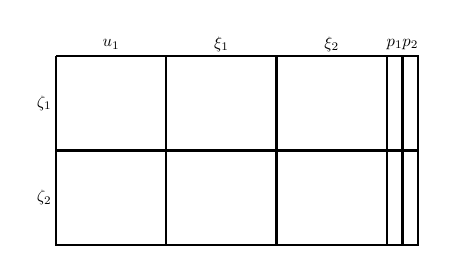
\begin{tikzpicture}[yscale=-1] 

\pgfmathsetmacro{\nt}{7};% time points
\pgfmathsetmacro{\ntm}{\nt-1};
\pgfmathsetmacro{\nu}{1}; % controls
\pgfmathsetmacro{\nx}{2}; % states
\pgfmathsetmacro{\np}{2}; % parameters
\pgfmathsetmacro{\nc}{\nu + \nx}; % total continuous

%% control labels
\foreach \k in {1,...,\nu}{
	\pgfmathsetmacro{\x}{0.2*\nt*\k - 0.2/2*(\nt-1)};
	\node () at (\x,-0.05) {\scalebox{0.6}{$u_{\k}$}};
}

%% state labels
\foreach \k in {1,...,\nx}{
	\pgfmathsetmacro{\x}{0.2*\nt*\k + 0.2*\nu*\nt - 0.2/2*(\nt-1)};
	\node () at (\x,-0.05) {\scalebox{0.6}{$\xi_{\k}$}};
}

%% parameter labels
\foreach \k in {1,...,\np}{
	\pgfmathsetmacro{\x}{0.2*\k + 0.2*\nu*\nt + 0.2*\nx*\nt};
	\node () at (\x,-0.05) {\scalebox{0.6}{$p_{\k}$}};
}

%% defects
\foreach \k in {1,...,\nx}{
	\pgfmathsetmacro{\x}{0.2*\ntm*\k - 0.2/2*(\ntm-1)};
	\node () at (-0.05,\x) {\scalebox{0.6}{$\zeta_{\k}$}};
}


%% controls
\foreach \k in {1,...,\nu}{
	\foreach \j in {1,...,\nx}{
		\foreach \i in {1,...,\ntm}{ 
        	\pgfmathsetmacro{\kk}{\k-1};
            \pgfmathsetmacro{\jj}{\j-1};
        	\pgfmathsetmacro{\x}{0.2*\i + 0.2*\kk*\nt};
            \pgfmathsetmacro{\y}{0.2*\i + 0.2*\jj*\ntm};
        	\node () at (\x,\y) {\mysparsesymbol};
            \node () at (\x+0.2,\y) {\mysparsesymbol};
} 
    \pgfmathsetmacro{\kk}{\k-1};
    \pgfmathsetmacro{\jj}{\j-1};
    \pgfmathsetmacro{\x}{0.2*\kk*\nt + 0.1};
    \pgfmathsetmacro{\y}{0.2*\jj*\ntm + 0.1};
	\draw[\mysparseboxcolor,thick](\x,\y) -- (\x+0.2*\nt,\y) -- (\x+0.2*\nt,\y+0.2*\ntm) -- (\x,\y+0.2*\ntm) -- (\x,\y);
} }

%% states
\foreach \k in {1,...,\nx}{
	\foreach \j in {1,...,\nx}{
		\foreach \i in {1,...,\ntm}{ 
        	\pgfmathsetmacro{\kk}{\k-1};
            \pgfmathsetmacro{\jj}{\j-1};
        	\pgfmathsetmacro{\x}{0.2*\i + 0.2*\nu*\nt + 0.2*\kk*\nt};
            \pgfmathsetmacro{\y}{0.2*\i + 0.2*\jj*\ntm};
        	\node () at (\x,\y) {\mysparsesymbol};
            \node () at (\x+0.2,\y) {\mysparsesymbol};
} 
    \pgfmathsetmacro{\kk}{\k-1};
    \pgfmathsetmacro{\jj}{\j-1};
    \pgfmathsetmacro{\x}{0.2*\kk*\nt + 0.2*\nu*\nt + 0.1};
    \pgfmathsetmacro{\y}{0.2*\jj*\ntm + 0.1};
	\draw[\mysparseboxcolor,thick](\x,\y) -- (\x+0.2*\nt,\y) -- (\x+0.2*\nt,\y+0.2*\ntm) -- (\x,\y+0.2*\ntm) -- (\x,\y);
} }

%% states and parameters
\foreach \k in {1,...,\np}{
	\foreach \j in {1,...,\nx}{
		\foreach \i in {1,...,\ntm}{ 
        	\pgfmathsetmacro{\kk}{\k-1};
            \pgfmathsetmacro{\jj}{\j-1};
        	\node () at ( 0.2*\k + 0.2*\nx*\nt + 0.2*\nu*\nt, 0.2*\i + 0.2*\jj*\ntm ) {\mysparsesymbol};
} 
    \pgfmathsetmacro{\kk}{\k-1};
    \pgfmathsetmacro{\jj}{\j-1};
    \pgfmathsetmacro{\x}{0.2*\kk + 0.2*\nx*\nt + 0.2*\nu*\nt + 0.1};
    \pgfmathsetmacro{\y}{0.2*\jj*\ntm+ 0.1};
	\draw[\mysparseboxcolor,thick](\x,\y) -- (\x+0.2,\y) -- (\x+0.2,\y+0.2*\ntm) -- (\x,\y+0.2*\ntm) -- (\x,\y);
} }

%% states
\foreach \k in {1,...,\nx}{
	\foreach \j in {1,...,\nx}{
		\foreach \i in {1,...,\ntm}{ 
        	\pgfmathsetmacro{\kk}{\k-1};
            \pgfmathsetmacro{\jj}{\j-1};
        	\pgfmathsetmacro{\x}{0.2*\i + 0.2*\nu*\nt + 0.2*\kk*\nt};
            \pgfmathsetmacro{\y}{0.2*\i + 0.2*\jj*\ntm};
            \node () at (\x+0.2,\y) {\mytemp};
} } }

\end{tikzpicture}
}
% 	\end{minipage}
% }%
% \subfloat[(c) $\bm{\theta}_3$ terms.]{
% 	\begin{minipage}{0.33\textwidth}
% 	\tikzsetnextfilename{ASSTheta3}

\centering
\resizebox{1\textwidth}{!}{
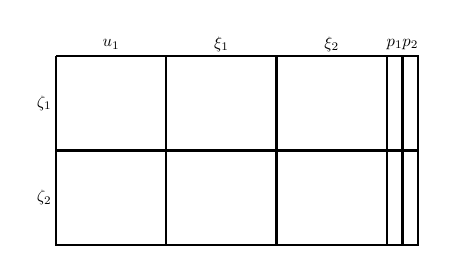
\begin{tikzpicture}[yscale=-1] 

\pgfmathsetmacro{\nt}{7};% time points
\pgfmathsetmacro{\ntm}{\nt-1};
\pgfmathsetmacro{\nu}{1}; % controls
\pgfmathsetmacro{\nx}{2}; % states
\pgfmathsetmacro{\np}{2}; % parameters
\pgfmathsetmacro{\nc}{\nu + \nx}; % total continuous

%% control labels
\foreach \k in {1,...,\nu}{
	\pgfmathsetmacro{\x}{0.2*\nt*\k - 0.2/2*(\nt-1)};
	\node () at (\x,-0.05) {\scalebox{0.6}{$u_{\k}$}};
}

%% state labels
\foreach \k in {1,...,\nx}{
	\pgfmathsetmacro{\x}{0.2*\nt*\k + 0.2*\nu*\nt - 0.2/2*(\nt-1)};
	\node () at (\x,-0.05) {\scalebox{0.6}{$\xi_{\k}$}};
}

%% parameter labels
\foreach \k in {1,...,\np}{
	\pgfmathsetmacro{\x}{0.2*\k + 0.2*\nu*\nt + 0.2*\nx*\nt};
	\node () at (\x,-0.05) {\scalebox{0.6}{$p_{\k}$}};
}

%% defects
\foreach \k in {1,...,\nx}{
	\pgfmathsetmacro{\x}{0.2*\ntm*\k - 0.2/2*(\ntm-1)};
	\node () at (-0.05,\x) {\scalebox{0.6}{$\zeta_{\k}$}};
}


%% controls
\foreach \k in {1,...,\nu}{
	\foreach \j in {1,...,\nx}{
		\foreach \i in {1,...,\ntm}{ 
        	\pgfmathsetmacro{\kk}{\k-1};
            \pgfmathsetmacro{\jj}{\j-1};
        	\pgfmathsetmacro{\x}{0.2*\i + 0.2*\kk*\nt};
            \pgfmathsetmacro{\y}{0.2*\i + 0.2*\jj*\ntm};
        	\node () at (\x,\y) {\mysparsesymbol};
            \node () at (\x+0.2,\y) {\mysparsesymbol};
} 
    \pgfmathsetmacro{\kk}{\k-1};
    \pgfmathsetmacro{\jj}{\j-1};
    \pgfmathsetmacro{\x}{0.2*\kk*\nt + 0.1};
    \pgfmathsetmacro{\y}{0.2*\jj*\ntm + 0.1};
	\draw[\mysparseboxcolor,thick](\x,\y) -- (\x+0.2*\nt,\y) -- (\x+0.2*\nt,\y+0.2*\ntm) -- (\x,\y+0.2*\ntm) -- (\x,\y);
} }

%% states
\foreach \k in {1,...,\nx}{
	\foreach \j in {1,...,\nx}{
		\foreach \i in {1,...,\ntm}{ 
        	\pgfmathsetmacro{\kk}{\k-1};
            \pgfmathsetmacro{\jj}{\j-1};
        	\pgfmathsetmacro{\x}{0.2*\i + 0.2*\nu*\nt + 0.2*\kk*\nt};
            \pgfmathsetmacro{\y}{0.2*\i + 0.2*\jj*\ntm};
        	\node () at (\x,\y) {\mysparsesymbol};
            \node () at (\x+0.2,\y) {\mysparsesymbol};
} 
    \pgfmathsetmacro{\kk}{\k-1};
    \pgfmathsetmacro{\jj}{\j-1};
    \pgfmathsetmacro{\x}{0.2*\kk*\nt + 0.2*\nu*\nt + 0.1};
    \pgfmathsetmacro{\y}{0.2*\jj*\ntm + 0.1};
	\draw[\mysparseboxcolor,thick](\x,\y) -- (\x+0.2*\nt,\y) -- (\x+0.2*\nt,\y+0.2*\ntm) -- (\x,\y+0.2*\ntm) -- (\x,\y);
} }

%% states and parameters
\foreach \k in {1,...,\np}{
	\foreach \j in {1,...,\nx}{
		\foreach \i in {1,...,\ntm}{ 
        	\pgfmathsetmacro{\kk}{\k-1};
            \pgfmathsetmacro{\jj}{\j-1};
        	\node () at ( 0.2*\k + 0.2*\nx*\nt + 0.2*\nu*\nt, 0.2*\i + 0.2*\jj*\ntm ) {\mysparsesymbol};
} 
    \pgfmathsetmacro{\kk}{\k-1};
    \pgfmathsetmacro{\jj}{\j-1};
    \pgfmathsetmacro{\x}{0.2*\kk + 0.2*\nx*\nt + 0.2*\nu*\nt + 0.1};
    \pgfmathsetmacro{\y}{0.2*\jj*\ntm+ 0.1};
	\draw[\mysparseboxcolor,thick](\x,\y) -- (\x+0.2,\y) -- (\x+0.2,\y+0.2*\ntm) -- (\x,\y+0.2*\ntm) -- (\x,\y);
} }

%% controls
\foreach \k in {1,...,\nu}{
	\foreach \j in {1,...,\nx}{
		\foreach \i in {1,...,\ntm}{ 
        	\pgfmathsetmacro{\kk}{\k-1};
            \pgfmathsetmacro{\jj}{\j-1};
        	\pgfmathsetmacro{\x}{0.2*\i + 0.2*\kk*\nt};
            \pgfmathsetmacro{\y}{0.2*\i + 0.2*\jj*\ntm};
        	\node () at (\x,\y) {\mytemp};
} } }

\end{tikzpicture}
}
% 	\end{minipage}
% }%

% \subfloat[(d) $\bm{\theta}_4$ terms.]{
% 	\begin{minipage}{0.33\textwidth}
% 	\tikzsetnextfilename{ASSTheta4}

\centering
\resizebox{1\textwidth}{!}{
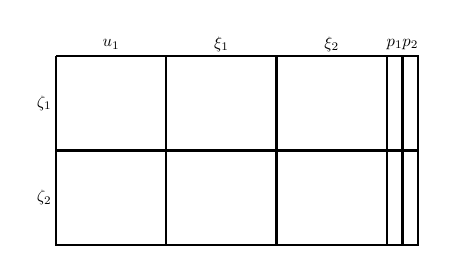
\begin{tikzpicture}[yscale=-1] 

\pgfmathsetmacro{\nt}{7};% time points
\pgfmathsetmacro{\ntm}{\nt-1};
\pgfmathsetmacro{\nu}{1}; % controls
\pgfmathsetmacro{\nx}{2}; % states
\pgfmathsetmacro{\np}{2}; % parameters
\pgfmathsetmacro{\nc}{\nu + \nx}; % total continuous

%% control labels
\foreach \k in {1,...,\nu}{
	\pgfmathsetmacro{\x}{0.2*\nt*\k - 0.2/2*(\nt-1)};
	\node () at (\x,-0.05) {\scalebox{0.6}{$u_{\k}$}};
}

%% state labels
\foreach \k in {1,...,\nx}{
	\pgfmathsetmacro{\x}{0.2*\nt*\k + 0.2*\nu*\nt - 0.2/2*(\nt-1)};
	\node () at (\x,-0.05) {\scalebox{0.6}{$\xi_{\k}$}};
}

%% parameter labels
\foreach \k in {1,...,\np}{
	\pgfmathsetmacro{\x}{0.2*\k + 0.2*\nu*\nt + 0.2*\nx*\nt};
	\node () at (\x,-0.05) {\scalebox{0.6}{$p_{\k}$}};
}

%% defects
\foreach \k in {1,...,\nx}{
	\pgfmathsetmacro{\x}{0.2*\ntm*\k - 0.2/2*(\ntm-1)};
	\node () at (-0.05,\x) {\scalebox{0.6}{$\zeta_{\k}$}};
}


%% controls
\foreach \k in {1,...,\nu}{
	\foreach \j in {1,...,\nx}{
		\foreach \i in {1,...,\ntm}{ 
        	\pgfmathsetmacro{\kk}{\k-1};
            \pgfmathsetmacro{\jj}{\j-1};
        	\pgfmathsetmacro{\x}{0.2*\i + 0.2*\kk*\nt};
            \pgfmathsetmacro{\y}{0.2*\i + 0.2*\jj*\ntm};
        	\node () at (\x,\y) {\mysparsesymbol};
            \node () at (\x+0.2,\y) {\mysparsesymbol};
} 
    \pgfmathsetmacro{\kk}{\k-1};
    \pgfmathsetmacro{\jj}{\j-1};
    \pgfmathsetmacro{\x}{0.2*\kk*\nt + 0.1};
    \pgfmathsetmacro{\y}{0.2*\jj*\ntm + 0.1};
	\draw[\mysparseboxcolor,thick](\x,\y) -- (\x+0.2*\nt,\y) -- (\x+0.2*\nt,\y+0.2*\ntm) -- (\x,\y+0.2*\ntm) -- (\x,\y);
} }

%% states
\foreach \k in {1,...,\nx}{
	\foreach \j in {1,...,\nx}{
		\foreach \i in {1,...,\ntm}{ 
        	\pgfmathsetmacro{\kk}{\k-1};
            \pgfmathsetmacro{\jj}{\j-1};
        	\pgfmathsetmacro{\x}{0.2*\i + 0.2*\nu*\nt + 0.2*\kk*\nt};
            \pgfmathsetmacro{\y}{0.2*\i + 0.2*\jj*\ntm};
        	\node () at (\x,\y) {\mysparsesymbol};
            \node () at (\x+0.2,\y) {\mysparsesymbol};
} 
    \pgfmathsetmacro{\kk}{\k-1};
    \pgfmathsetmacro{\jj}{\j-1};
    \pgfmathsetmacro{\x}{0.2*\kk*\nt + 0.2*\nu*\nt + 0.1};
    \pgfmathsetmacro{\y}{0.2*\jj*\ntm + 0.1};
	\draw[\mysparseboxcolor,thick](\x,\y) -- (\x+0.2*\nt,\y) -- (\x+0.2*\nt,\y+0.2*\ntm) -- (\x,\y+0.2*\ntm) -- (\x,\y);
} }

%% states and parameters
\foreach \k in {1,...,\np}{
	\foreach \j in {1,...,\nx}{
		\foreach \i in {1,...,\ntm}{ 
        	\pgfmathsetmacro{\kk}{\k-1};
            \pgfmathsetmacro{\jj}{\j-1};
        	\node () at ( 0.2*\k + 0.2*\nx*\nt + 0.2*\nu*\nt, 0.2*\i + 0.2*\jj*\ntm ) {\mysparsesymbol};
} 
    \pgfmathsetmacro{\kk}{\k-1};
    \pgfmathsetmacro{\jj}{\j-1};
    \pgfmathsetmacro{\x}{0.2*\kk + 0.2*\nx*\nt + 0.2*\nu*\nt + 0.1};
    \pgfmathsetmacro{\y}{0.2*\jj*\ntm+ 0.1};
	\draw[\mysparseboxcolor,thick](\x,\y) -- (\x+0.2,\y) -- (\x+0.2,\y+0.2*\ntm) -- (\x,\y+0.2*\ntm) -- (\x,\y);
} }

%% controls
\foreach \k in {1,...,\nu}{
	\foreach \j in {1,...,\nx}{
		\foreach \i in {1,...,\ntm}{ 
        	\pgfmathsetmacro{\kk}{\k-1};
            \pgfmathsetmacro{\jj}{\j-1};
        	\pgfmathsetmacro{\x}{0.2*\i + 0.2*\kk*\nt};
            \pgfmathsetmacro{\y}{0.2*\i + 0.2*\jj*\ntm};
            \node () at (\x+0.2,\y) {\mytemp};
} } }

\end{tikzpicture}
}
% 	\end{minipage}
% }%
% \subfloat[(e) $\bm{\theta}_5$ terms.]{
% 	\begin{minipage}{0.33\textwidth}
% 	\tikzsetnextfilename{ASSTheta5}

\centering
\resizebox{1\textwidth}{!}{
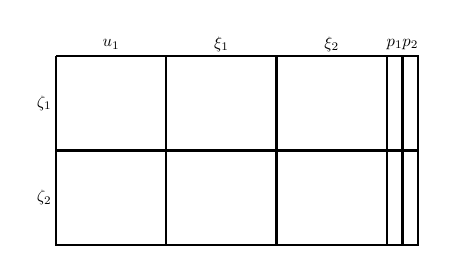
\begin{tikzpicture}[yscale=-1] 

\pgfmathsetmacro{\nt}{7};% time points
\pgfmathsetmacro{\ntm}{\nt-1};
\pgfmathsetmacro{\nu}{1}; % controls
\pgfmathsetmacro{\nx}{2}; % states
\pgfmathsetmacro{\np}{2}; % parameters
\pgfmathsetmacro{\nc}{\nu + \nx}; % total continuous

%% control labels
\foreach \k in {1,...,\nu}{
	\pgfmathsetmacro{\x}{0.2*\nt*\k - 0.2/2*(\nt-1)};
	\node () at (\x,-0.05) {\scalebox{0.6}{$u_{\k}$}};
}

%% state labels
\foreach \k in {1,...,\nx}{
	\pgfmathsetmacro{\x}{0.2*\nt*\k + 0.2*\nu*\nt - 0.2/2*(\nt-1)};
	\node () at (\x,-0.05) {\scalebox{0.6}{$\xi_{\k}$}};
}

%% parameter labels
\foreach \k in {1,...,\np}{
	\pgfmathsetmacro{\x}{0.2*\k + 0.2*\nu*\nt + 0.2*\nx*\nt};
	\node () at (\x,-0.05) {\scalebox{0.6}{$p_{\k}$}};
}

%% defects
\foreach \k in {1,...,\nx}{
	\pgfmathsetmacro{\x}{0.2*\ntm*\k - 0.2/2*(\ntm-1)};
	\node () at (-0.05,\x) {\scalebox{0.6}{$\zeta_{\k}$}};
}


%% controls
\foreach \k in {1,...,\nu}{
	\foreach \j in {1,...,\nx}{
		\foreach \i in {1,...,\ntm}{ 
        	\pgfmathsetmacro{\kk}{\k-1};
            \pgfmathsetmacro{\jj}{\j-1};
        	\pgfmathsetmacro{\x}{0.2*\i + 0.2*\kk*\nt};
            \pgfmathsetmacro{\y}{0.2*\i + 0.2*\jj*\ntm};
        	\node () at (\x,\y) {\mysparsesymbol};
            \node () at (\x+0.2,\y) {\mysparsesymbol};
} 
    \pgfmathsetmacro{\kk}{\k-1};
    \pgfmathsetmacro{\jj}{\j-1};
    \pgfmathsetmacro{\x}{0.2*\kk*\nt + 0.1};
    \pgfmathsetmacro{\y}{0.2*\jj*\ntm + 0.1};
	\draw[\mysparseboxcolor,thick](\x,\y) -- (\x+0.2*\nt,\y) -- (\x+0.2*\nt,\y+0.2*\ntm) -- (\x,\y+0.2*\ntm) -- (\x,\y);
} }

%% states
\foreach \k in {1,...,\nx}{
	\foreach \j in {1,...,\nx}{
		\foreach \i in {1,...,\ntm}{ 
        	\pgfmathsetmacro{\kk}{\k-1};
            \pgfmathsetmacro{\jj}{\j-1};
        	\pgfmathsetmacro{\x}{0.2*\i + 0.2*\nu*\nt + 0.2*\kk*\nt};
            \pgfmathsetmacro{\y}{0.2*\i + 0.2*\jj*\ntm};
        	\node () at (\x,\y) {\mysparsesymbol};
            \node () at (\x+0.2,\y) {\mysparsesymbol};
} 
    \pgfmathsetmacro{\kk}{\k-1};
    \pgfmathsetmacro{\jj}{\j-1};
    \pgfmathsetmacro{\x}{0.2*\kk*\nt + 0.2*\nu*\nt + 0.1};
    \pgfmathsetmacro{\y}{0.2*\jj*\ntm + 0.1};
	\draw[\mysparseboxcolor,thick](\x,\y) -- (\x+0.2*\nt,\y) -- (\x+0.2*\nt,\y+0.2*\ntm) -- (\x,\y+0.2*\ntm) -- (\x,\y);
} }

%% states and parameters
\foreach \k in {1,...,\np}{
	\foreach \j in {1,...,\nx}{
		\foreach \i in {1,...,\ntm}{ 
        	\pgfmathsetmacro{\kk}{\k-1};
            \pgfmathsetmacro{\jj}{\j-1};
        	\node () at ( 0.2*\k + 0.2*\nx*\nt + 0.2*\nu*\nt, 0.2*\i + 0.2*\jj*\ntm ) {\mysparsesymbol};
} 
    \pgfmathsetmacro{\kk}{\k-1};
    \pgfmathsetmacro{\jj}{\j-1};
    \pgfmathsetmacro{\x}{0.2*\kk + 0.2*\nx*\nt + 0.2*\nu*\nt + 0.1};
    \pgfmathsetmacro{\y}{0.2*\jj*\ntm+ 0.1};
	\draw[\mysparseboxcolor,thick](\x,\y) -- (\x+0.2,\y) -- (\x+0.2,\y+0.2*\ntm) -- (\x,\y+0.2*\ntm) -- (\x,\y);
} }

%% states and parameters
\foreach \k in {1,...,\np}{
	\foreach \j in {1,...,\nx}{
		\foreach \i in {1,...,\ntm}{ 
        	\pgfmathsetmacro{\kk}{\k-1};
            \pgfmathsetmacro{\jj}{\j-1};
        	\node () at ( 0.2*\k + 0.2*\nx*\nt + 0.2*\nu*\nt, 0.2*\i + 0.2*\jj*\ntm ) {\mytemp};
} } }

\end{tikzpicture}
}
% 	\end{minipage}
% }%

% \caption{Sparsity pattern of $\mathbf{A}_{e1}$ matrix for the defect constraints using a single-step method.}\label{fig:figsparsityASS}
% \end{figure}